% Resultate
\section{Resultate}

\subsection{Kort}
\textsc{Kort} besteht aus fünf verschiedenen Hauptmasken.
Diese sind in der Applikation über die Tabs im unteren Bereich erreichbar.

\subsubsection{Maske: Aufträge}
In dieser Maske werden dem Benutzer alle noch nicht gelösten Fehler in seiner Umgebung als Markierungen auf der Karte angezeigt.
Die Fehleranzahl ist dabei auf die 25 nächstgelegenen Fehler limitiert.

Beim Klick auf einen Fehler wird der Benutzer gefragt, ob er diesen auch wirklich lösen kann.
Bestätigt er wird ihm der Fehler im Detail angezeigt.
In dieser Detailansicht wir ihm zudem je nach Fehlertyp ein Text- oder ein Auswahlfeld angezeigt in welchem er die Antwort eingeben bzw. auswählen kann. 

Zusätzlich hat er die Möglichkeit sich den Fehler nochmals auf der Karte anzuzeigen zu lassen.
Dabei wird dieser nicht nur als Markierung dargestellt sondern als ein Geometrie-Objekt entsprechend den OpenStreetMap-Daten.
Eine Strasse wird dabei beispielsweise als Linie dargestellt und ein Gelände als Polygon.

\begin{figure}[H]
\subfigure{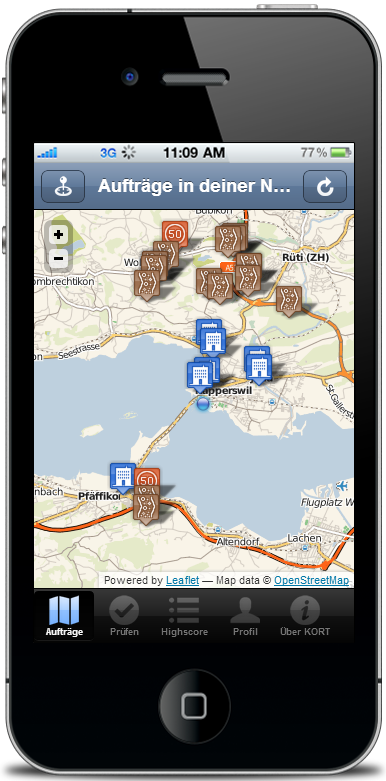
\includegraphics[width=0.3\textwidth]{images/screenshots/kort-screenshot-bugmap}}
\hfill
\subfigure{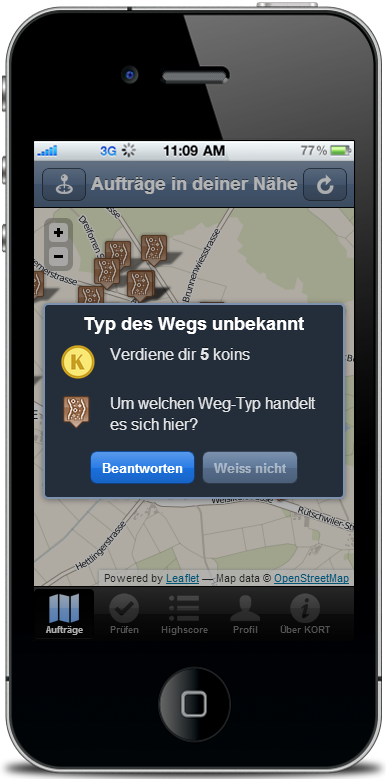
\includegraphics[width=0.3\textwidth]{images/screenshots/kort-screenshot-bugmap_message_box}}
\hfill
\subfigure{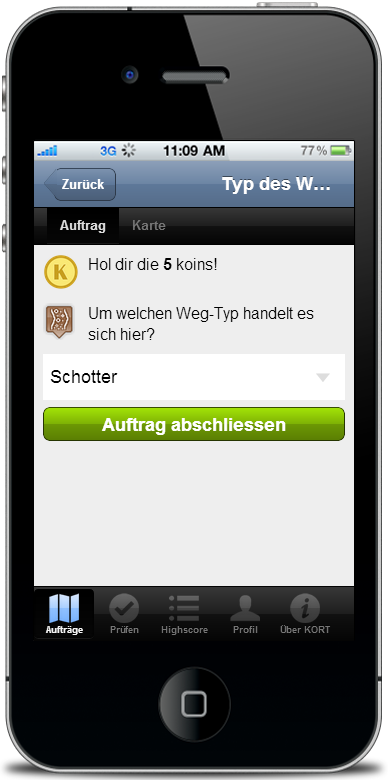
\includegraphics[width=0.3\textwidth]{images/screenshots/kort-screenshot-fix}}
\caption{Maske: Aufträge}
\end{figure}

\subsubsection{Maske: Prüfen}
In der Prüfen-Maske werden dem Benutzer die Lösungen angezeigt, welche noch zu überprüfen sind.
Diese sind dabei nach der Anzahl noch nötiger positiver Überprüfungen gruppiert.
So soll erreicht werden, dass Lösungen die schon bald an OpenStreetMap zurückgesendet werden können bevorzugt behandelt werden.
In der Liste werden maximal 25 Überprüfungen angezeigt.

Sobald er einen Eintrag anklickt, wird ihm der Fehler auf der Karte angezeigt inklusiver der eingetragenen Lösung.
Er kann nun beurteilen, ob ihm diese Lösung korrekt oder eher falsch erscheint.

\begin{figure}[H]
\subfigure{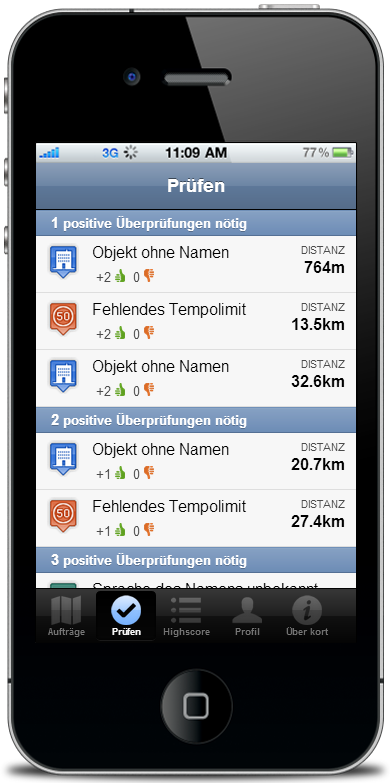
\includegraphics[width=0.3\textwidth]{images/screenshots/kort-screenshot-validation}}
\hfill
\subfigure{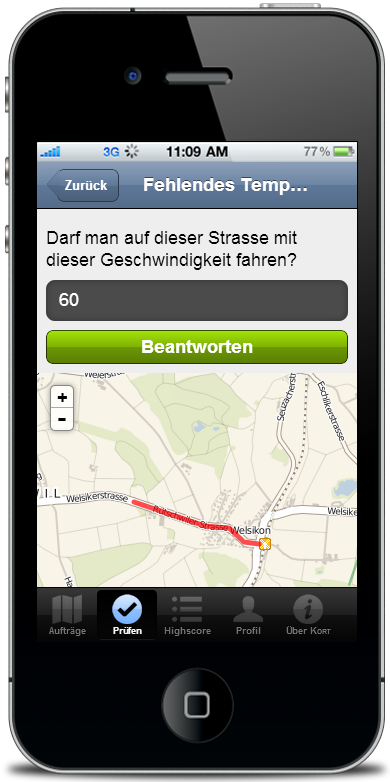
\includegraphics[width=0.3\textwidth]{images/screenshots/kort-screenshot-vote}}
\hfill
\subfigure{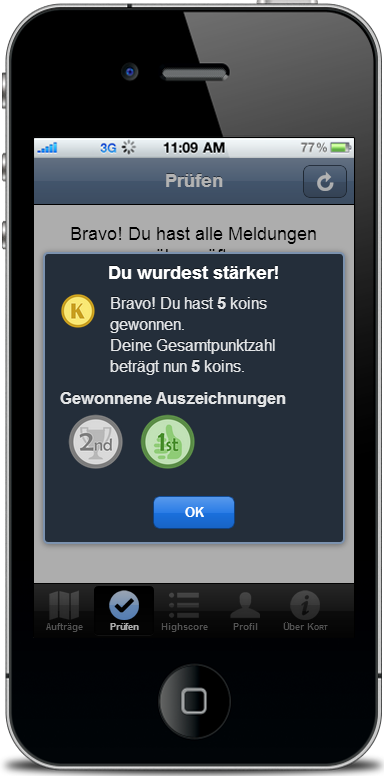
\includegraphics[width=0.3\textwidth]{images/screenshots/kort-screenshot-reward}}
\caption{Maske: Prüfen}
\end{figure}

\subsubsection{Maske: Highscore}
In der Highscore werden die Benutzer abhängig der Anzahl von ihnen gewonnener Punkte (sog. \emph{koins}) sortiert.
Es werden jeweils die ersten zehn Platzierungen angezeigt. Falls man selbst nicht zu diesen gehört wird zusätzlich eine Zeile mit seiner eigenen Platzierung angezeigt.

\subsubsection{Maske: Profil}
Im Profil findet man eine Zusammenfassung seiner persönlichen Spielaktivitäten.
Man sieht die Gesamtanzahl der gesammelten \emph{koins} und eine Übersicht der gewonnen Auszeichnungen

\subsubsection{Maske: Über Kort}
Auf der \emph{Über Kort}-Seite werden allgemeine Informationen zur Applikation angezeigt.

\begin{figure}[H]
\subfigure{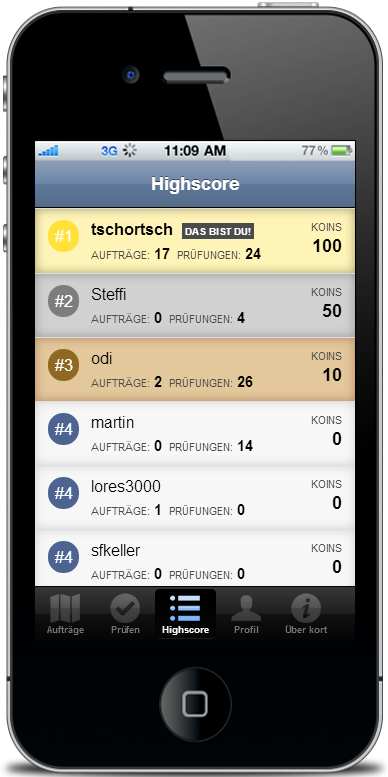
\includegraphics[width=0.3\textwidth]{images/screenshots/kort-screenshot-highscore}}
\hfill
\subfigure{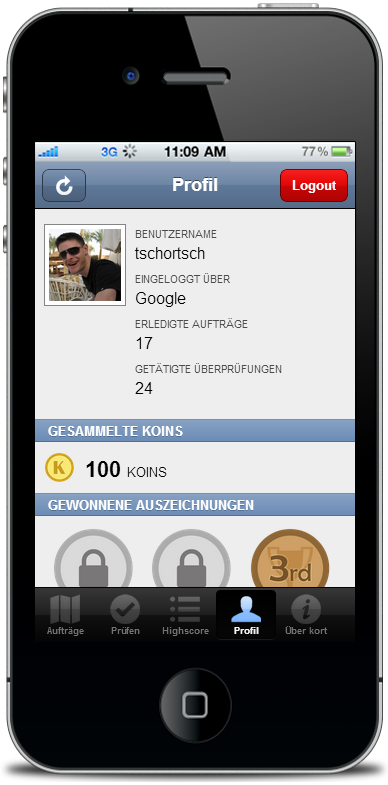
\includegraphics[width=0.3\textwidth]{images/screenshots/kort-screenshot-profile}}
\hfill
\subfigure{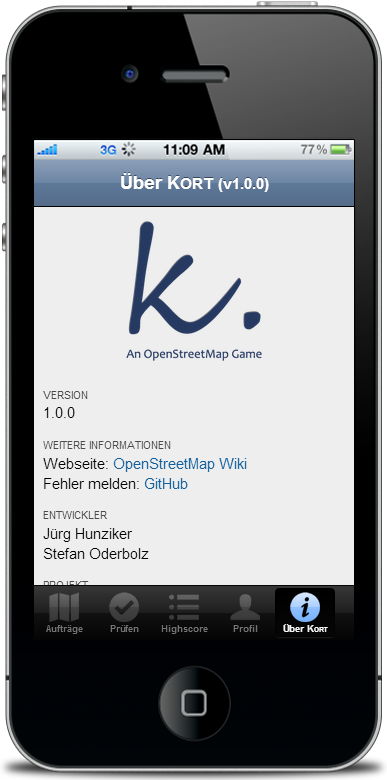
\includegraphics[width=0.3\textwidth]{images/screenshots/kort-screenshot-about}}
\caption{Masken: Highscore / Profil / Über Kort}
\end{figure}

\subsection{Bekannte Fehler}

\subsubsection{iOS6 - Add to homescreen}
Eine sehr nützliche Funktionalität, welche Apple im Mobile Safari-Browser anbietet ist die \emph{Add to homescreen}-Funktion.

\begin{figure}[H]
\subfigure{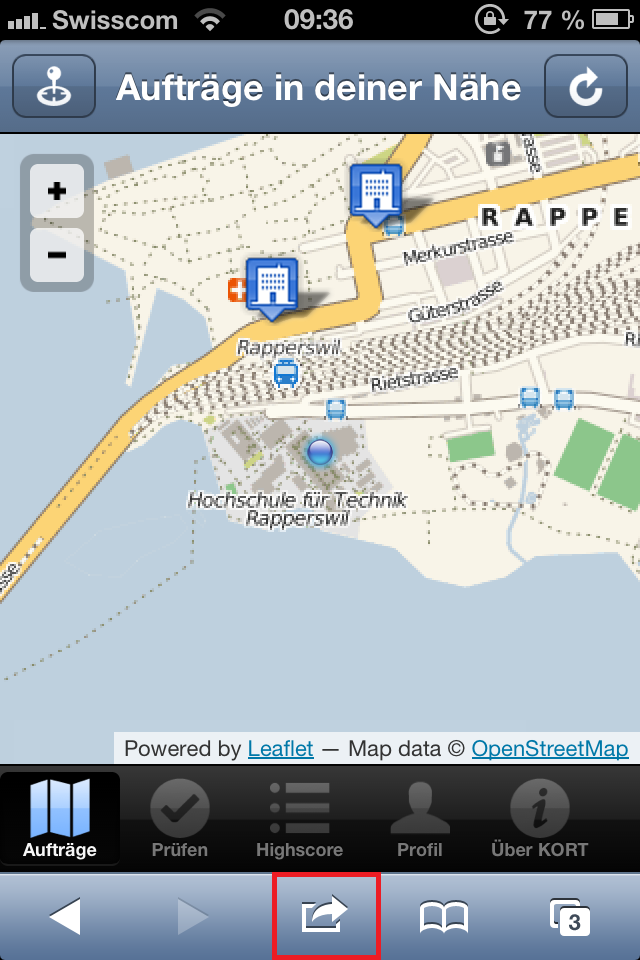
\includegraphics[width=0.23\textwidth]{images/bugs/kort-add_to_homescreen_1}}
\hfill
\subfigure{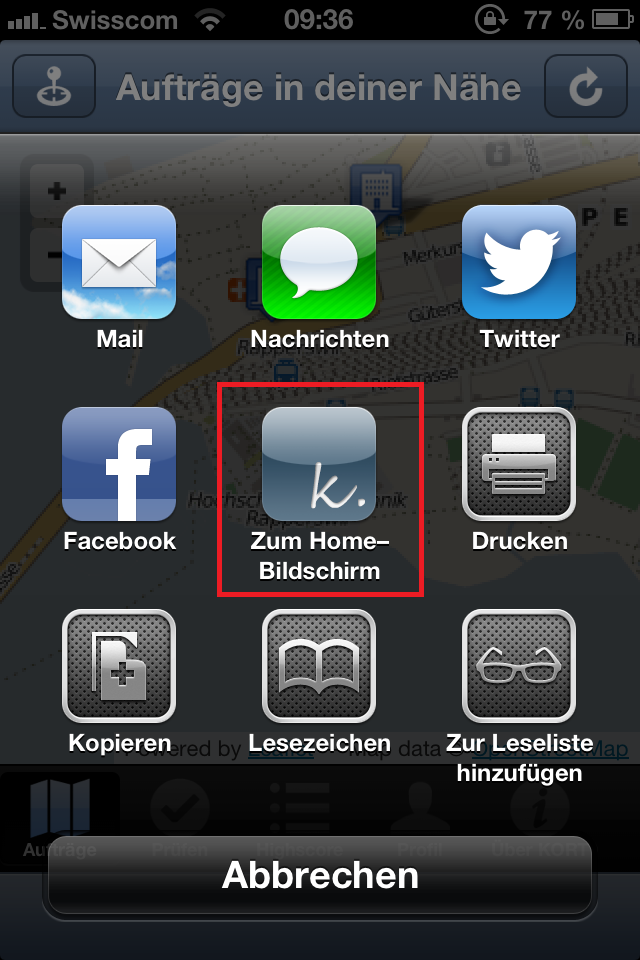
\includegraphics[width=0.23\textwidth]{images/bugs/kort-add_to_homescreen_2}}
\hfill
\subfigure{
\includegraphics[width=0.23\textwidth]{images/bugs/kort-add_to_homescreen_3}}
\hfill
\subfigure{
\includegraphics[width=0.23\textwidth]{images/bugs/kort-add_to_homescreen_4}}
\caption{iOS - "`Add to homescreen"'-Funktion}
\end{figure}

Dadurch wird ein App-ähnlicher Bookmark der aktuellen Webseite auf dem Homescreen erstellt.
Dieser erhält ein hinterlegtes Icon und einen Titel.
Beim Starten der App erscheint ein Splashscreen, welchen man ebenfalls in der Webseite definieren kann.
Zudem öffnet sich der Browser ohne jegliche Toolbars wie der Adressleiste oder der Navigationsbar.

Leider befindet in iOS6 ein Bug, welcher den Zugriff auf die Geolocation verhindert, wenn die \gls{WebApp} vom Homescreen aus gestartet wird.
Auf Stack Overflow\footnote{\url{http://stackoverflow.com/questions/12503815/ios-6-breaks-geolocation-in-webapps-apple-mobile-web-app-capable}} wird der Bug genauer beschrieben.

\textbf{Workaround}

Im Sencha Fourm\footnote{\url{http://www.sencha.com/forum/showthread.php?246317-2.1.0-RC1-Save-to-home-screen-Geolocation-not-working}} wird als Workaround vorgeschlagen die Generierung des folgenden Metatags (siehe Code-Ausschnitt \ref{code-ios6-homescreen-metatag}) in der Sencha Touch Library zu deaktivieren.

\lstset{language=HTML}
\begin{lstlisting}[caption=Metatag für iOS6 Workaround, label=code-ios6-homescreen-metatag]
<meta content="yes" name="apple-mobile-web-app-capable" />
\end{lstlisting}

Diese befindet sich in folgenden Dateien:

\begin{itemize}
\item \inlinecode{/touch/microloader/development.js} Zeile 24
\item \inlinecode{/touch/microloader/production.js} Zeile 564
\item \inlinecode{/touch/microloader/testing.js} Zeile 24
\item \inlinecode{/touch/sencha-touch-all-debug.js} Zeile 9345
\item \inlinecode{/touch/sencha-touch-debug.js} Zeile 9345
\item \inlinecode{/touch/src/core/Ext-more.js} Zeile 657
\end{itemize}

Das Deaktivieren dieser Zeile hat aber zur Folge, dass der native Rahmen des Browsers (Adressleiste, Navigationsbar) wieder angezeigt wird.
Dies ist zwar unschön löst aber das Problem mit dem Zugriff auf die Geolocation.

\subsubsection{App Build}
Wie in Abschnitt \ref{sencha-cmd} beschrieben, basiert die App vollständig auf dem Sencha-eigenen Build-Tool \emph{Sencha Cmd 3.0.0.250}. Darin sind aber noch einige Bugs vorhanden.

Bei \textsc{Kort} besteht dabei ein Problem bei der fest eingebauten Komprimierung der JavaScript-Sourcen.
Während diesem Prozess werden lokale Variablennamen mit einzelnen Buchstaben abgekürzt.
Dabei treten Konflikte mit der Leaflet-Library auf, welche den Buchstaben \emph{L} als Namespace verwendet.

\textbf{Workaround}

Um diese Problem zu umgehen, mussten wir das Build-Skript von Sencha Cmd minimal anpassen.
So mussten wir die Zeile, welche den \gls{Microloader} komprimiert auskommentieren (siehe Code-Ausschnitt \ref{senchacmd-workaround}).
Diese befindet sich in folgender Datei:

\inlinecode{/<Sencha Cmd Verzeichnis>/plugins/touch/current/app-build.js} Zeile 362

\lstset{language=JavaScript}
\begin{lstlisting}[float, caption=Sencha Cmd Workaround, label=senchacmd-workaround]
processIndex = function () {
	[...]
	
	compressor = new ClosureCompressor();
	microloader = (environment == 'production'
		? 'production'
		: 'testing') +
		'.js';
	_logger.debug("using microloader : {}", microloader);
	content = readFileContent(joinPath(sdk, "microloader", microloader));
	//content = compressor.compress(content);
	remotes = [
		'<script type="text/javascript">' +
			content + ';Ext.blink(' +
			(environment == 'production' ? jsonEncode({
				id:config.id
			}) : appJson) + ')' +
			'</script>'
	];
	
	[...]
};
\end{lstlisting}